%% -*- coding: utf-8 -*-
\documentclass[12pt,a4paper]{scrartcl} 
\usepackage[utf8]{inputenc}
\usepackage[english,russian]{babel}
\usepackage{indentfirst}
\usepackage{misccorr}
\usepackage{graphicx}
\usepackage{amsmath}
\begin{document}

% Что должно быть во введении
\begin{enumerate}
\end{enumerate}
\large\tableofcontents

\vspace{25\baselineskip}

\section{Теория}
\subsection{Техническое задание}
\textbf {Задание:}

Вычислить матрицу обратную заданной.

\subsection{Теоретическая часть}

Алгоритм нахождения обратной матрицы методом исключения неизвестных Гаусса

1. К матрице A приписать единичную матрицу того же порядка.

2. Полученную сдвоенную матрицу преобразовать так, чтобы в левой её части получилась единичная матрица, тогда в правой части на месте единичной матрицы автоматически получится обратная матрица. Матрица A в левой части преобразуется в единичную матрицу путём элементарных преобразований матрицы.

3. Если в процессе преобразования матрицы A в единичную матрицу в какой-либо строке или в каком-либо столбце окажутся только нули, то определитель матрицы равен нулю, и, следовательно, матрица A будет вырожденной, и она не имеет обратной матрицы. В этом случае дальнейшее нахождение обратной матрицы прекращается.

\section{Ход работы}
\label{sec:exp}

\subsection{Код приложения}
\label{sec:exp:code}
\begin{verbatim}
import numpy as np

# задаем исходную матрицу
A = np.array([[2, 5, 7], [6, 3, 4], [5, -2, -3]])

# вычисляем обратную матрицу
A_inv = np.linalg.inv(A)

# выводим результат
print("Исходная матрица:\n", A)
print("Обратная матрица:\n", A_inv)
        \end{verbatim}


\subsection{Работа программы} 



\begin{wrapfigure}
  \begin{center}
    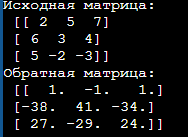
\includegraphics[width=0.5\textwidth]{matrix.jpg}
  \end{center}
  \caption{Рис.1  Пример работы программы.}\label{fig:ex}
\end{wrapfigure}

\newpage
\begin{thebibliography}{9}
\bibitem{Knuth-2003}Кнут Д.Э. Всё про \TeX. \newblock --- Москва: Изд. Вильямс, 2003 г. 550~с.
\bibitem{Lvovsky-2003}Львовский С.М. Набор и верстка в системе \LaTeX{}. \newblock --- 3-е издание, исправленное и дополненное, 2003 г.
\bibitem{Voroncov-2005}Воронцов К.В. \LaTeX{} в примерах. 2005 г.
\end{thebibliography}

\end{document}